
\documentclass[letterpaper,english,10pt]{article}

\usepackage{%
	amsfonts,%
	amsmath,%	
	amssymb,%
	amsthm,%
	babel,%
	bbm,%
	%biblatex,%
	caption,%
	centernot,%
	color,%
	enumerate,%
	%enumitem,%
	epsfig,%
	epstopdf,%
	etex,%
	fancybox,%
	framed,%
	fullpage,%
	%geometry,%
	graphicx,%
	hyperref,%
	latexsym,%
	mathptmx,%
	mathtools,%
	multicol,%
	pgf,%
	pgfplots,%
	pgfplotstable,%
	pgfpages,%
	proof,%
	psfrag,%
	%subfigure,%	
	tikz,%
	times,%
	ulem,%
	url,%
	xcolor,%
	mathpazo
}

\definecolor{shadecolor}{gray}{.95}%{rgb}{1,0,0}
\usepackage[margin=1in,top=0.75in]{geometry}
\usepackage[mathscr]{eucal}
\usepgflibrary{shapes}
\usepgfplotslibrary{fillbetween}
\usetikzlibrary{%
  arrows,%
  backgrounds,%
  chains,%
  decorations.pathmorphing,% /pgf/decoration/random steps | erste Graphik
  decorations.text,% 
  matrix,%
  positioning,% wg. " of "
  fit,%
  patterns,%
  petri,%
  plotmarks,%
  scopes,%
  shadows,%
  shapes.misc,% wg. rounded rectangle
  shapes.arrows,%
  shapes.callouts,%
  shapes%
}

%\pgfplotsset{compat=newest} %<------ Here
\pgfplotsset{compat=1.11} %<------ Or use this one

\theoremstyle{plain}
\newtheorem{thm}{Theorem}[section]
\newtheorem{lem}[thm]{Lemma}
\newtheorem{prop}[thm]{Proposition}
\newtheorem{cor}[thm]{Corollary}
\newtheorem{clm}[thm]{Claim}

\theoremstyle{definition}
\newtheorem{axiom}[thm]{Axiom}
\newtheorem{defn}[thm]{Definition}
\newtheorem{conj}[thm]{Conjecture}
\newtheorem{exmp}[thm]{Example}
\newtheorem{exerc}[thm]{Exercise}
\newtheorem{assum}[thm]{Assumptions}

\theoremstyle{remark}
\newtheorem{rem}[thm]{Remark}
\newtheorem{note}[thm]{Note}

\newcommand{\Cov}{\operatorname{Cov}}
%\newcommand{\det}{\operatorname{det}}
\newcommand{\Real}{\mathbb{R}}
\newcommand{\tr}{\operatorname{tr}}
%\newcommand{\Var}{\operatorname{Var}}

\DeclareMathOperator{\sign}{sign}
%\renewcommand{\proof}[1]{\begin{proof}#1\end{proof}}
\newcommand{\EQ}[1]{\begin{equation*}#1\end{equation*}}
\newcommand{\EQN}[1]{\begin{equation}#1\end{equation}}
\newcommand{\eq}[1]{\begin{align*}#1\end{align*}}
\newcommand{\meq}[2]{\begin{xalignat*}{#1}#2\end{xalignat*}}
\newcommand{\norm}[1]{\left\lVert#1\right\rVert}
\newcommand{\abs}[1]{\left\lvert#1\right\rvert}
\newcommand{\expect}[1]{\mathbb{E}\left[{#1}\right]}
\newcommand{\prob}[1]{\mathbb{P}\left[{#1}\right]}
\newcommand{\given}{\; \big\vert \;} 
\newcommand{\set}[1]{\left\{#1\right\}} 
\newcommand{\indicator}[1]{\mathbb{1}_{\set{#1}}} 
\newcommand{\inner}[1]{\left\langle#1\right\rangle}
\newcommand{\red}[1]{\textcolor{red}{#1}} 
\newcommand{\E}[1]{\mathbb{E}\left[#1\right]}
\newcommand{\Var}[1]{\operatorname{Var}\left[#1\right]}

\newcommand{\D}{\mathbb{D}}
%\newcommand{\E}{\mathbb{E}}
\newcommand{\N}{\mathbb{N}}
\renewcommand{\P}{\mathbb{P}}
\newcommand{\Q}{\mathbb{Q}}
\newcommand{\R}{\mathbb{R}}
\newcommand{\Z}{\mathbb{Z}}

\newcommand{\bU}{\mathbf{1}}
\newcommand{\bx}{\mathbf{x}}

\newcommand{\cB}{\mathcal{B}}
\newcommand{\cC}{\mathcal{C}}
\newcommand{\cD}{\mathcal{D}}
\newcommand{\cF}{\mathcal{F}}
\newcommand{\cG}{\mathcal{G}}
\newcommand{\cH}{\mathcal{H}}
\newcommand{\cO}{\mathcal{O}}
\newcommand{\cT}{\mathcal{T}}
\newcommand{\cX}{\mathcal{X}}
\newcommand{\cY}{\mathcal{Y}}

\newcommand{\sA}{\mathscr{A}}
\newcommand{\sB}{\mathscr{B}}
\newcommand{\sC}{\mathscr{C}}
\newcommand{\sD}{\mathscr{D}}
\newcommand{\sE}{\mathscr{E}}
\newcommand{\sF}{\mathscr{F}}
\newcommand{\sG}{\mathscr{G}}
\newcommand{\sH}{\mathscr{H}}
\newcommand{\sL}{\mathscr{L}}
\newcommand{\dO}{\mathscr{O}}
\newcommand{\sS}{\mathscr{S}}
\newcommand{\sT}{\mathscr{T}}
\newcommand{\sX}{\mathscr{X}}
\newcommand{\sY}{\mathscr{Y}}
\newcommand{\sZ}{\mathscr{Z}}

% Debug
\newcommand{\todo}[1]{\begin{color}{blue}{{\bf~[TODO:~#1]}}\end{color}}

% a few handy macros

\renewcommand{\le}{\leqslant}
\renewcommand{\ge}{\geqslant}
\newcommand\matlab{{\sc matlab}}
\newcommand{\goto}{\rightarrow}
\newcommand{\bigo}{{\mathcal O}}
%\newcommand{\half}{\frac{1}{2}}
%\newcommand\implies{\quad\Longrightarrow\quad}
\newcommand\reals{{{\rm l} \kern -.15em {\rm R} }}
\newcommand\complex{{\raisebox{.043ex}{\rule{0.07em}{1.56ex}} \hskip -.35em {\rm C}}}


% macros for matrices/vectors:

% matrix environment for vectors or matrices where elements are centered
\newenvironment{mat}{\left[\begin{array}{ccccccccccccccc}}{\end{array}\right]}
\newcommand\bcm{\begin{mat}}
\newcommand\ecm{\end{mat}}

% matrix environment for vectors or matrices where elements are right justifvied
\newenvironment{rmat}{\left[\begin{array}{rrrrrrrrrrrrr}}{\end{array}\right]}
\newcommand\brm{\begin{rmat}}
\newcommand\erm{\end{rmat}}

% for left brace and a set of choices
%\newenvironment{choices}{\left\{ \begin{array}{ll}}{\end{array}\right.}
\newcommand\when{&\text{if~}}
\newcommand\otherwise{&\text{otherwise}}
% sample usage:
%  \delta_{ij} = \begin{choices} 1 \when i=j, \\ 0 \otherwise \end{choices}


% for labeling and referencing equations:
\newcommand{\eql}{\begin{equation}\label}
\newcommand{\eqn}[1]{(\ref{#1})}
% can then do
%  \eql{eqnlabel}
%  ...
%  \end{equation}
% and refer to it as equation \eqn{eqnlabel}.  


% some useful macros for finite difference methods:
\newcommand\unp{U^{n+1}}
\newcommand\unm{U^{n-1}}

% for chemical reactions:
\newcommand{\react}[1]{\stackrel{K_{#1}}{\rightarrow}}
\newcommand{\reactb}[2]{\stackrel{K_{#1}}{~\stackrel{\rightleftharpoons}
   {\scriptstyle K_{#2}}}~}


\makeatletter
\def\th@plain{%
  \thm@notefont{}% same as heading font
  \itshape % body font
}
\def\th@definition{%
  \thm@notefont{}% same as heading font
  \normalfont % body font
}
\makeatother
\date{}

\graphicspath{{./Figures/}}
%\usepackage{witharrows}

\usepackage{multirow}
 \usepackage{booktabs}
%opening
\title{Lecture-24: Game Theory,Statistical Mechanics,Income Inequality} 
\author{Vivek VP}

\begin{document}
\maketitle
\section{Problem of income inequality}
\cite{fairgame}
Income inequality has been a growing concern in recent years. For example as of 2010, the top 1\% of households in the US owned 35.4 \% of all privately held wealth. This was just 20\% in 1976. Taking a look at India's situation; as per 2016 statistics,India is the second most unequal country in the world. Top 1\% rich people of India holds 58.4\% of wealth. These statistics show how severe is the wealth inequality and income inequality. There are many causes for this including poor infrastructure in rural areas. These have serious impact on living conditions of poor people. Poor people is denied access to good health and education which in turn turns this inequality to a social level. All this happens despite India's GDP is increasing faster than many countries of comparable scenario.

\section{Free market}
In a free market laws of supply and demand is free from any external intervention like government agencies. This includes an employer can hire and fire employees and employees can take new offers from a different employer if there is a better utility. 

\section{Income inequality in pay distribution}
Let us now focus on  the inequality in pay scale of employees in an organization. As of 2009 top 1\% of income earners received 17.2\% if income. Fundamental to solving this problem is understanding why this occurs. Clearly different employees make different contributions and this implies a certain amount of  inequality in income and wealth has to be expected. So we can ask the question what is a fair inequality? What kind of pay distribution will arise, under ideal conditions in a free market where employers are seeking profit maximization and employees are seeking utility maximization?

\section{Connection between statistical physics and income inequality problem}
There has been a lot of effort to model income and wealth distributions by applying statistical physics method. But appreciating those efforts there is still a conceptual gap between them. How will a theory of random particles with no intelligence be able to model a environment that consists of rational profit seeking agents? 

\section{Game Theory}
We will use theory of potential games as a tool for getting the equilibrium of income inequality problem. So lets take a brief introduction to game theory. \\
Game theory is the study of mathematical models for strategic interaction between rational and intelligent agents. There are different types of games. Let us look at the one relevant to us which is strategic form games. Let us discuss a bit on what terms rational and intelligent means:

\begin{defn}
Strategic Form Game: A strategic form game $\Gamma$ is a tuple $\langle N, (S_i)_{i\in N}, (u_i)_{i \in N} \rangle$ , where 
\begin{itemize}
\item $N = \lbrace 1,2,\dots ,n\rbrace$ is set of players;
\item $S_1,S_2,\dots S_n$ are sets called the strategy sets of the players $1,\dots , n$ respectively; and
\item Set of strategy profiles $S$ is the cartesian product of individual strategy sets $S=\lbrace s_1 \times s_2 \times s_N : s_1\in S_1, s_2 \in S_2 \dots s_N \in S_N  \rbrace $
\item $u_i  : S \rightarrow \R$ for $i=1,2,\dots n$ are mappings called the utility functions or payoff functions.

\end{itemize}
 \end{defn}
\begin{exmp}
$ N=\lbrace 1,2 \rbrace ;S_1= S_2 = \lbrace A,B \rbrace ;$ \\ \\
$u_1(A,A) = 10; u_1(A,B)=0; u_1(B,A) = 0 ; u_1(B.B) = 1;$ \\ \\
$u_2(A,A) = 10; u_2(A,B)=0; u_2(B,A) = 0 ; u_2(B.B) = 1;$ \\ \\
\end{exmp}
Payoff functions of a player is not just dependent on his strategy but also on what strategies others are playing.
Above example can be put in a tabular form

\begin{table}[ht]
\begin{center}
\begin{tabular}{|c|c|c|}
\hline
\multirow{2}{*}{1} & \multicolumn{2}{c|}{2} \\ \cline{2-3} 
                   & A           & B        \\ \hline
A                  & 10,10       & 0,0      \\ \hline
B                  & 0,0         & 1,1      \\ \hline
\end{tabular}
\end{center}
\end{table}







Here first value in payoff cell stands for first player and second value stands for second player.
\begin{defn}
Potential Game: A strategic form game is a potential game if there exists a function $\phi:S \to R $ such that 
\begin{equation} \label{pgt}
\phi(S')-\phi(S'') = u_i(S') - u_i(S'')~~
\forall~i , \forall S', S'' \in 
\end{equation}
\end{defn}

This means if we know $\phi$ we know the payoff matrix upto a offset. 
\begin{thm}\label{pgtne}
	In a potenital game strategy profile maximizing $\phi$ is a Nash equilbria.
\end{thm}
\begin{proof}
	Now consider two strategy $s'$ and $s''$ profiles which differs only in strategy for player $i$.Also assume $s'$ maximizes $\phi$. So $\phi(s')-\phi(s'')>0$ . But from $\ref{pgt}$ we have $u_i(s')-u_i(s'')>0 \forall i$ Hence $s'$ is a Nash equilbria.
\end{proof}
So in potential game theory all we need to find a Nash equilbria is to maximize $\phi$ 
\begin{exmp}
	Consider a game and its potential $\phi$, assuming $\phi(A,A)=0$
		\begin{table}[ht]
	\begin{minipage}{0.5\textwidth}
	\begin{center}
		\begin{tabular}{|c|c|c|}
			\hline
			\multirow{2}{*}{1} & \multicolumn{2}{c|}{2} \\ \cline{2-3} 
			& A           & B        \\ \hline
			A                  & 1,2       & 2,3     \\ \hline
			B                  & 4,5        & 6,7     \\ \hline
		\end{tabular}
	\label{game2}
	\caption{Game}
		\end{center}
	\end{minipage}
\begin{minipage}{0.5\textwidth}
	\begin{center}
		\begin{tabular}{|c|c|c|}
			\hline
			\multirow{2}{*}{1} & \multicolumn{2}{c|}{2} \\ \cline{2-3} 
			& A           & B        \\ \hline
			A                  & 0     & 1      \\ \hline
			B                  & 3        & 5    \\ \hline
		\end{tabular}
	\label{potential2}
	\caption{potential}
	\end{center}
\end{minipage}
\end{table}

\end{exmp}


\section{Dynamics} \cite{fairentrop}
 Consider a company $A$ with:
\begin{enumerate}
	 \item Total salary budget $M$ 
	 \item Total number of employees $N$
	 \item $k$ levels of employment with value $v_i$ for $i^{th}$ level.Assume $v_i < v_j$ for $i<j$
	 For example level $1$ could be a clerk and level $k$ be CEO.
\end{enumerate}

For our market we assume a simplified model of all companies have same  slary budget and total number of employees and number of levels of employment. Also assume market is a \textbf{free market}.

Let us look at an example.
\begin{figure}[h!]
	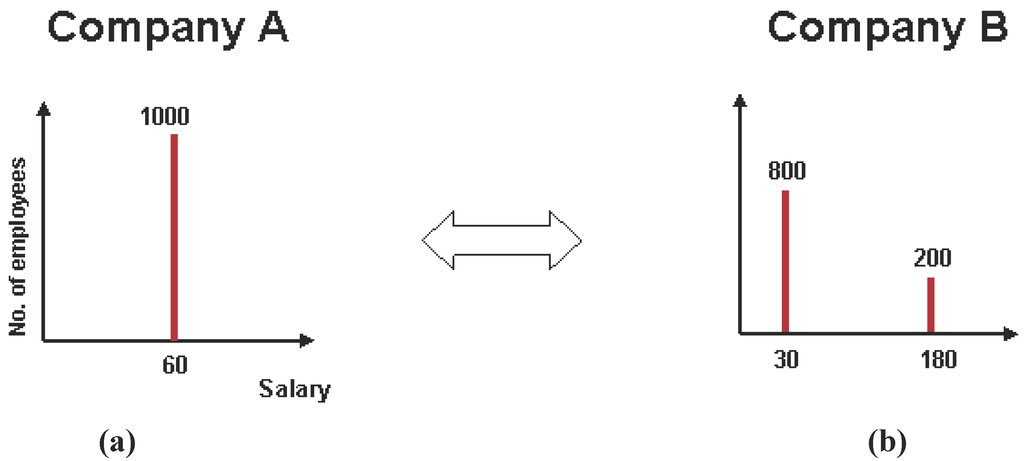
\includegraphics[width=\linewidth]{dynamics1.png}
	\caption{Initial distribution}
	\label{fig:1}
\end{figure}

Consider two companies A and B with 3 different levels of employment with $v1<v2<v3$; call it low skill, medium skill, high skill.
Both A and B have $\text{total number of employees} ~ N =1000$ and $\text{total salary budget}~ M=\$60~ \text{million dollar}$ with initial distribution as shown in Figure1 \ref{fig:1}.

\begin{figure}[h!] \label{fig2}
	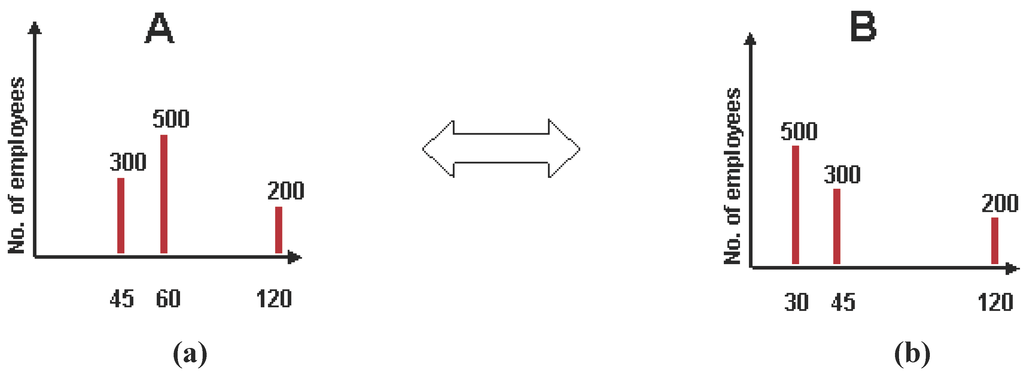
\includegraphics[width=\linewidth]{dynamics2.png}
	\caption{Evolving}
	\label{fig:2}
\end{figure}

 Now highly skilled employees in company A are not satisfied; so they try to jump to $B$. Now $B$ is also trying to make profit out of this situation. So $B$ doesn't want to give the same salary of $180$  to highly skilled employees from $A$. But highly skilled employees from $A$ and $B$ will have a negotiation and say they settle for $120$. Now highly skilled employees of $A$ will be ready to work for $120$. Hence a new level will be formed both in $A$ and $B$ of $120$. Now distribtuion will look as given in Figure2 \ref{fig:2}.





\begin{figure}[h!] \label{fig3}
	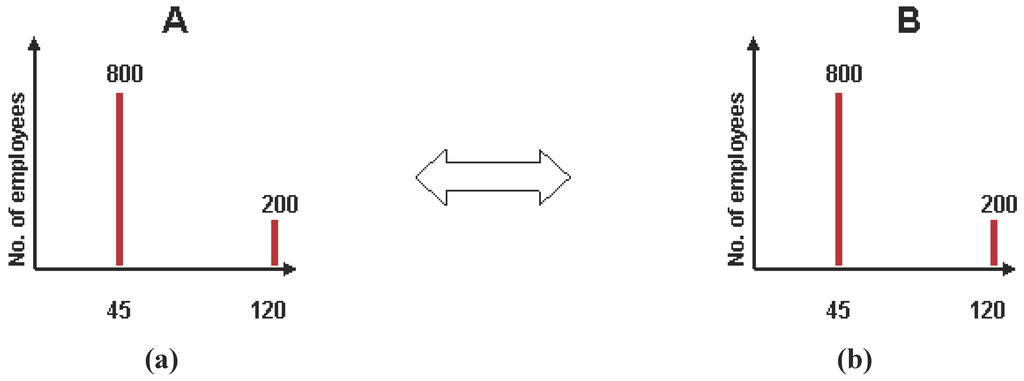
\includegraphics[width=\linewidth]{dynamics3.png}
	\caption{After evolution}
	\label{fig:Earthatmo}
\end{figure}

So this is the dynamics we are talking about.


\section{Setting the payoff or utility}
In general an employee feels they could be doing better given their talent and experience. Utility maximizing, fairness-seeking, teleological agents are always restless. Even though utility obtained by an employee is a complex aggregate, we formulate it as obtained from 3 major factors. 
\begin{itemize}
    \item Utility derived from salary.
    \item Disutility from effort
    \item Utility from fairness.
    
\end{itemize}
\subsection{A note on fairness}
Employees are looking for fair compensation for their abilities and contribution to the organization. This will depend on the education and other qualifications the possess. But an employee is looking for appreciation with respect to peers at his level. This means a clerk is not eyeing for the post of a CEO. Similarly a a vice president is not happy if he gets more salary than a clerk. But he expects to get utility on par with other vice presidents. So that means utility from fairness is a function only of number of employees at his level ($N_i$) . 
\subsection{Functional form for utility terms}
So we can write \\
$h_i(S_i,E_i,N_i) = u(S_i) - v(E_i) + f(N_i)$
$h_i$ : is the total utility of an employee earning a salary $S_i$ by expending an effort $E_i$ while competing with $(N_i -1) $ other agents. \\

Now we need to come up with functional form for each of the three terms $u,v,f$ \\
Let us consider the following empirical and theoretical considerations from literature regarding effort $E$ and salary $S$.
\begin{itemize}
\item Salary
 \begin{itemize}
    \item Logarithmic function is commonly used in literature for utility from salary. 
       
    \item This gives $u(S_i) = \alpha ln S_i$
       
   \end{itemize}
\item Effort 
   \begin{itemize}
    \item  Work by Katz \cite{katz} and Akerlof \cite{akerlof} gives following conditions to be satisfied by effort $E$ as a function of salary $S$
    \begin{itemize}
        \item $dE/dS >0$
        \item $E(0) \leq 0 $
        \item the elasticity $S/E \times (dE/dS)$ should be decreasing.
    \end{itemize}
    \item Empirical evidence that supports effort $E$ correlates with $lnS$ ; $E= lnS$; given in Stratton \cite{stratton} and Ahituv and Lerman \cite{ahituv}. This goes well with previous point because: \\
     \begin{itemize}
     \item $\frac{dE}{dS} = \frac{1}{S} >0$
     \item $E(0) = -\inf < 0$
     \item $S/E \times (\frac{dE}{dS}) = (\frac{S}{ln S}) \times \frac{1}{S} = \frac{1}{ln S} $ is decreasing.
     \end{itemize}
     \item Hence $v(E_i) = \beta (ln S_i)^2$
   \end{itemize}
   \item Fairness 
        \begin{itemize}
        \item We propose $f(N_i) = -\gamma~ ln N_i$
        \item We note following observations are captured in this form
           \begin{itemize}
               \item As $N_i \to \inf $, $f_i \to -inf$; this captures the idea that when there are too many employees working with a person his appreciation is minimized.
               \item When $N_i = 0, f_i \to \inf. $ This explains why employees are in constant search of their dream jobs. When $N_i=0$ , this is when utility from fairness is maximized mathematically; but this cannot be attained in reality because minimum value of $N_i$ is 1 in reality (at least  oneself should be there).
           \end{itemize}
        \end{itemize}
   
\end{itemize}
Thus we have :
\begin{equation}
    u(S_i) = \alpha ln S_i
\end{equation}
\begin{equation}
    v(E_i) = \beta (ln S_i)^2
\end{equation}
\begin{equation}
f(N_i) = - \gamma ln N_i
\end{equation}
\begin{equation}\label{utility}
 h_i(S_i,E_i,N_i) = u(S_i) - v(E_i) + f(N_i)= \alpha ln S_i - \beta (ln S_i)^2 - \gamma ln N_i
 \end{equation}
\section{Applying potential game theory}
\begin{equation}
    h_i(x) \equiv  \frac{\partial\phi(x)}{\partial x_i}
\end{equation}
\begin{equation} \label{potential}
    \phi(x) = \sum_{i=1}^{n}\int{}{}h_i(x)dx_i
\end{equation}
\begin{equation}
    \phi(x) = \phi_u + \phi_v + \phi_f + constant ; where
\end{equation}
\begin{equation}
    \phi_u = \alpha \sum_{i=1}^{n}x_i lnS_i ;and
\end{equation}
\begin{equation}
    \phi_v = -\beta \sum_{i=1}^{n} x_i(ln S_i)^2 ; and
\end{equation}
\begin{equation}
    \phi_v = \gamma/N ln \frac{N!}{\prod_{j=1}^{n}(Nx_i)!}
\end{equation}
We can show that $\phi(x)$ is strictly concave: 
\begin{equation}
    \dfrac{\partial^2 \phi(x)}{\partial x_i^2}= \dfrac{-\gamma}{x_i}<0
\end{equation}
Therefore, a unique Nash equilbrium exists for this game; which is a maximizer for $\phi$ . \\
To find maximizer $x_i$
we use langrangian multiplier method with $L$ as langrangian and $\lambda$ as Langrange multiplier. Thus 
\begin{equation}
     L=\phi + \lambda(1-\sum_{i=1}{n}x_i)
\end{equation}
We solve system of equations given by
\begin{equation}
     \frac{\partial L}{\partial x_i} =0 ~ \forall i
 \end{equation}
 
 We get 
 \begin{equation}
    \alpha ln S_i-\beta (ln S_i)^2 - \gamma ln Nx_i - \lambda = 0
 \end{equation}
 giving
 \begin{equation}
     x_i = e ^ {\alpha ln S_i - \beta (ln S_i)^2 - \gamma ln N -\lambda}
 \end{equation}
 which can be rearranged to get
 
 \begin{equation}\label{fairpotential}
     x_i = \dfrac{1}{S_i Z}exp(-\dfrac{(lnS_i - \dfrac{\alpha+\gamma}{2\beta})^2 }{\dfrac{\gamma}{\beta}})
 \end{equation}
 where 
 \begin{equation}
     Z = N exp[\lambda/\gamma - \dfrac{(\alpha + \gamma)^2}{4\beta \gamma}]
 \end{equation}
 which is a \textbf{log-normal distribution}
 

\section{Deriving Boltzmann distribution using potential game theory}
Let us define the payoff of particles in the thermodynamic game:

\begin{equation}\label{thermogame}
    h_i(E_i,N_i) = -\beta E_i - ln N_i
\end{equation}
where $E_i$ is the energy of a molecule in state $i$, $\beta=\frac{1}{kT}$, $k=1.3806488 \times 10^{-23} JK^{-1}$ is Boltzmann constant; and $T$ is temperature.
 Now from \ref{potential} we have 
 \begin{equation}
 \phi(x) = \frac{-\beta}{N}+ \frac{1}{N}ln\frac{N!}{\prod_{i=1}^{n}(Nx_i)!}
 \end{equation}
 We need to maximize $\phi(x)$ under constraint $\sum_{j=1}{k}x_j = 1$.
 Using Langrange multiplier method with L as Langrangian we have
 \begin{equation}
     L=\phi + \lambda(1-\sum_{i=1}{n}x_i)
 \end{equation}
 For maximizing; we solve set of equations given by
 \begin{equation}
     \frac{\partial L}{\partial x_i} =0 ~ \forall i
 \end{equation}
 We get 
 \begin{equation}
     \beta E_i  - ln N - ln x_i -\lambda = 0 
 \end{equation}
 giving
 \begin{equation}
     x_i = e ^ {\beta E_i  - ln N  -\lambda}
 \end{equation}
 Also $\sum_{j=1}^{k}x_j=1$; which gives
 \begin{equation}
     x_i = \frac{x_i}{1} = \frac{x_i}{\sum_{j=1}^{k}x_j} = \frac{e ^ {\beta E_i  - ln N  -\lambda}}{\sum_{j=1}^{k}e ^ {\beta E_j  - ln N  -\lambda}}
 \end{equation}
 giving
 \begin{equation}
     x_i = \frac{e^{-\beta E_i}}{\sum_{j=1}^{k}e^{-\beta E_i}}
 \end{equation}
 which is nothing but \textbf{Boltzmann Distribution}
 
\section{Replicator Dynamics}
Consider the situation of people buying cars. We compare people buying an SUV and compact cars. Let us define the following payoff table constructed by considering the fact that when one SUV meets another SUV there is less space on road and less fuel efficiency. We consider  similar situation for an SUV and compact and compact and compact.

\begin{table}[ht]
\begin{center}
\begin{tabular}{|c|c|c|}
\hline
%\multirow{2}{*}{1} & \multicolumn{2}{c|}{2} \\ \cline{2-3} 
                   & SUV           & Compact        \\ \hline
SUV                 & 2,2       & 2,0      \\ \hline
Compact                  & 0,2         & 3,3      \\ \hline
\end{tabular}
\end{center}
\end{table}
As from the table it is observed that purchasing compact cars is better for users.But in reality number of SUVs are on rise. How do we explain this situation. But people are not purely rational. They have emotions and feelings as well.One thing they do out of emotions is to copy others. Also they are not completely out of rationality. So in  order to model this situation we use replicator dynamics.
This is a simple model of evolution and prestige based learning in games. We explain this model through an example\\ 
\subsection{Model Description through example}
Consider a population of $N$ people divided into $k$ classes . Let $x_i(t)$ be the fraction of people belonging to class $i$ at time epoch $t$.  Tuple $(x_1(t),\dots x_k(t))$ define the state of the population at time epoch $t$. $\pi_i(t)$ is the expected payoff for a player when randomly matched with another player. This is clearly a function of payoff matrix and state of population. \\
In the SUV and compact cars game if we have a population of $50\%$ SUVs and $50\%$ comapct cars, expected payoff for an compact car owner is \\
\begin{equation}
E=0.5\times U_c(C,C) + 0.5 \times U_s(C,S)
\end{equation}
$E=0.5\times U_c(C,C) + 0.5 \times U_s(C,S)$(C stands for compact and S stands for SUV) where $U_c$ is the utility function for compact.First term corresponds to $50\%$ chance of meeting an compact and similarly second term corresponds to $50\%$ chance of meeting an SUV. In the
Also we have $\sum_{i=0}^{k}x_i(t) = 1 ~~ \forall t$
Now we see the equation for evolution of population in replicator dynamics.
\begin{equation}
    x_i(t+1) = \frac{x_i(t)\pi_i(t)}{\sum_{j=i}^{k}x_j(t)\pi_j(t)}
\end{equation}
We calculate rate of change of $x_i$ i.e $x_i(t+1)-x_i(t)$  
\begin{equation}
    x_i(t+1) - x_i(t) =  \frac{x_i(t)\pi_i(t)}{\sum_{j=i}^{k}x_j(t)\pi_i(t)} -x_i(t)
    = \frac{x_i(t)(\pi_i(t)-\sum_{j=i}^{k}x_j(t)\pi_i(t)}{\sum_{j=i}^{k}x_j(t)\pi_i(t)}
\end{equation}
Denote by $\overset{.}x_i = x_i(t+1) - x_i(t)$, rate of change of $x_i$; 
We have
\begin{equation}
\overset{.}x_i \propto x_i(t)(\pi_i(t)-\sum_{j=i}^{k}x_j(t)\pi_j(t)) 
\end{equation}
We can interpret the term $\sum_{j=i}^{k}x_j(t)\pi_(t)$ as average payoff of the population. 

Under equilibrium we have $\overset{.}x_i =0 $  \\
 i.e 
 \begin{equation}\label{rdeqm}
    \pi_i(t)=\sum_{j=i}^{k}x_j(t)\pi_j(t)
 \end{equation} \\
 i.e payoff for a class is equal to average payoff under equilibrium.
 

 \section{Deriving equilibrium income distribution using replicator dynamics}
 From \ref{utility} and \ref{rdeqm} we have 
 \begin{equation}
     h_i = h^* ~\forall i ~\text{where $h^*$ is equilibrium payoff under replicator dynamics.} 
 \end{equation}
 \begin{equation}
     \alpha ln S_i - \beta (ln S_i)^2 -\gamma ln N_i = h^* 
 \end{equation}
 
 But $N_i = Nx_i$
 
 \begin{equation}
     \alpha ln S_i - \beta (ln S_i)^2 -\gamma ln Nx_i = h^* 
 \end{equation}
 
 Solving for $x_i$
 
 \begin{equation}
     x_i = e^{\alpha ln S_i - \beta (ln S_i)^2 -\gamma ln N - h^*}
 \end{equation}
 which can be rearranged to get 
 \begin{equation}\label{fairrd}
     x_i = \dfrac{1}{S_i Z}exp(-\dfrac{(lnS_i - \dfrac{\alpha+\gamma}{2\beta})^2 }{\dfrac{\gamma}{\beta}})
 \end{equation}
 where 
 \begin{equation}
     Z = N exp[h^*/\gamma - \dfrac{(\alpha + \gamma)^2}{4\beta \gamma}]
 \end{equation}
 We recognize that \ref{fairrd} is a \textbf{log-normal distribution}.
 \section{Deriving Boltzmann distribution using replicator dynamics }
     Under equilibrium ; from \ref{rdeqm} and \ref{thermogame} we have 
     \begin{equation}
         -\beta E_i -ln(Nx_i) = h^*
     \end{equation}
     Giving
     \begin{equation}
         x_i = e^{-\beta E_i -ln N -h^*}
     \end{equation}
     Also $\sum_{j=1}^{k}x_j=1$; which gives
     \begin{equation}
         x_i = \frac{e^{-\beta E_i -ln N -h^*}}{\sum_{j=1}^{k}x_j} = \frac{e^{-\beta E_i}}{\sum_{j=1}^{k}e^{-\beta E_j}}
     \end{equation}
     which is nothing but Boltzmann distribution 
     
  \begin{thebibliography}{9}
  	
  	\bibitem{fairgame}
  	Venkat Venkatasubramanian, Yu~Luo, and Jay Sethuraman.
  	\newblock Game theory, statistical mechanics and income inequality.
  	\newblock {\em arXiv preprint arXiv:1406.6620}, 2014.
  	
  	\bibitem{fairentrop}
  	Venkat Venkatasubramanian.
  	\newblock Fairness is an emergent self-organized property of the free market
  	for labor.
  	\newblock {\em Entropy}, 12(6):1514--1531, 2010.
  	
    \bibitem{katz}
    Lawrence~F. Katz.
    \newblock Efficiency wage theories: A partial evaluation.
    \newblock {\em NBER Macroeconomics Annual}, 1:235--276, 1986.
  	
  	\bibitem{akerlof}
  	George~A Akerlof and Janet~L Yellen.
  	\newblock {\em Efficiency wage models of the labor market}.
  	\newblock Cambridge University Press, 1986.
  	
  
  	
  	
  	
  	\bibitem{stratton}
  	Leslie~S Stratton.
  	\newblock Why does more housework lower women's wages? testing hypotheses
  	involving job effort and hours flexibility.
  	\newblock {\em Social Science Quarterly}, 82(1):67--76, 2001.
  	
  	\bibitem{ahituv}
  	Avner Ahituv and Robert~I. Lerman.
  	\newblock How do marital status, work effort, and wage rates interact?
  	\newblock {\em Demography}, 44(3):623--647, Aug 2007.
  	
  	
  	
  \end{thebibliography}
 %\bibliographystyle{unsrt}
 %\bibliography{lecture-25.bib}
 
 
%  $\bar{f}$
 

 

 
% \begin{itemize}

% \item Use the environment definitions for lemma, theorem, definition, proof, example, and other such environments you may need, wherever necessary. Usage of {\bf Definition} for a definition is not acceptable. Different environments are listed in this document below.
% \item Add the .tex file header in your latex file for the below commands to work (\textbackslash input\{header\}, second line of the source file sampleLecture.tex).
% \item Make sure that there are no spelling mistakes in the scribed notes.
% \item Use environments such as align, equation, eqnarray or gather to deal with multi-line equations, instead of newline characters. 
% \item Use punctuation in all equations.
% \item Always make sure that the lecture notes uploaded is complete.
% \item Any math symbol in a line should be within math environment \$\$. For example, \$Y\$ is used to write a math symbol $Y$.
% \item Revise your lectures before uploading, so that there no variations in the style in which the document is prepared.
% \item If you are using figures in the tex file, put them in the Figures folder.
% \item Please label and caption the figures.
% \item Use full sentences for captions as well, and even when writing equations.
% \item Motivate each section with a sentence or two, on why are we studying this?
% \end{itemize}
% \section{Examples usage of environments}
% \begin{itemize}
% \item Equation with multiple cases:
% \begin{equation}
% A = 
% \begin{cases}
% 1 &if~TRUE\\
% 0 &if~FALSE.
% \end{cases}
% \end{equation}
% \item Theorem:
% \begin{thm}
% Theorem goes here
% \end{thm}
% \item Corollary:
% \begin{cor}
% content...
% \end{cor}
% \item Proposition:
% \begin{prop}
% content...
% \end{prop}
% \item Lemma:
% \begin{lem}
% content...
% \end{lem}
% \item Definition:
% \begin{defn}
% Definition
% \end{defn}
% \item Conjecture:
% \begin{conj}
% Content...
% \end{conj}
% \item Example:
% \begin{exmp}
% Content...
% \end{exmp}
% \item Assumptions:
% \begin{assum}
% Content...
% \end{assum}
% \item Axiom:
% \begin{axiom}
% Content...
% \end{axiom}
% \item Remark:
% \begin{rem}
% Content...
% \end{rem}
% \item Note:
% \begin{note}
% This is a note.
% \end{note}
% \end{itemize}
% \begin{note}
% Scribed notes that does not follow the guidelines mentioned above attracts penalty.
% \end{note}
\end{document}